\chapter{Reflexão Crítica e Problemas Encontrados}
\label{chap:reflexao}

\section{Introdução}
\label{chap4:sec:intro}

Não obstante o bom planeamento feito a priori na fase de engenharia de \emph{software} (descrito no Capítulo \ref{ch::engsoft}), o projeto \emph{Challenge-Accepted}, tal como qualquer outro na área das \ac{TI}, enfrentou alguns contratempos e, com o tempo ao dispor, não se revelou possível almejar todas as ambições inicialmente imaginadas. É preciso, pois, refletir sobre o desenvolvimento deste projeto. 
    
    Neste Capítulo são, portanto, explorados os seguintes tópicos:
\begin{itemize}
\item Objetivos propostos vs. alcançados (Secção \ref{chap4:sec:opvsoa}): compara os objetivos
inicialmente propostos com aqueles que foram concluídos no projeto final;
\item Divisão de trabalho pelos elementos do grupo (Secção \ref{chap4:sec:divisao}): lista as tarefas
realizadas por cada elemento da equipa;
\item Problemas encontrados (Secção \ref{chap4:sec:problemas}): na sequência da Secção \ref{chap4:sec:opvsoa}, explora
os problemas encontrados durante a implementação da aplicação;
\item Reflexão crítica (Secção \ref{chap4:sec:reflexao}): é feita uma \ac{SWOT} em retrospetiva pela equipa acerca do projeto.
\end{itemize}

\section{Objetivos Propostos vs. Alcançados}
\label{chap4:sec:opvsoa}

\begin{table}[!htbp]
	\centering
	\begin{tabular}{p{.65\textwidth} >{\centering\let\newline\\\arraybackslash\hspace{0pt}}m{.25\textwidth}}
		\toprule
		{\bfseries Objetivo proposto} & {\bfseries Alcançado?} \\
		\midrule
		Registo de utilizadores com representação segura da palavra-passe na base de dados & $\bullet$ \\
		Submissão de desafios do tipo cifra de mensagens, codificando-a em \textit{BASE64} & $\bullet$ \\	
		Cálculo de código de autenticação de mensagens que permite verificar se uma mensagem foi bem decifrada ou não & $\bullet$ \\
		Submissão de desafios do tipo valor de \textit{hash}, codificando-a em \textit{BASE64} & $\bullet$ \\
		Resposta a desafios e verificação do sucesso da tentativa  & $\bullet$ \\
		Desafios com cifras AES-128-ECB, AES-128-CBC e AES-128-CTR & $\bullet$ \\
		Desafios com funções de hash MD5, SHA256 e SHA512          & $\bullet$ \\
		Limite de uma tentativa a cada 15 segundos para os desafios de cifra &  \\
		Verificar se uma mensagem foi bem decifrada através de assinaturas digitais RSA & - \\
		Suporte ao algoritmo El Gamal                                           & \\
		Outro tipo de desafios criptográficos                                   & \\
		\bottomrule
	\end{tabular}
	\caption[Objetivos propostos vs. alcançados]{
		Objetivos propostos e respetiva indicação de sucesso.\\
		\textit{Legenda.} $\bullet$ Alcançado em pleno; $\circ$ Alcançado parcialmente. -- Não alcançado.
	}
	\label{tab::objetivos}
\end{table}



\section{Divisão do Trabalho pelos Elementos do Grupo}
\label{chap4:sec:divisao}

\begin{table}[!htbp]
	\centering
	\begin{tabular}{l c c c c c}
		\toprule
		\textbf{Tarefa}                             & \textbf{DL} & \textbf{JA} & \textbf{DS} & \textbf{BC} & \textbf{IN} \\
		\midrule
		Gestão do projeto                           &             &             &             &              &            \\
		Engenharia de Software (requisitos)         &             &             &             &              &             \\
		Engenharia de Software (diagramas)          &             &             &             &              &             \\
		Instalação infraestrutura de suporte        &             &             &             &              &            \\
	    Desenvolvimento da base de dados            &             &             &             &              &            \\
		\textit{Framework} da aplicação (cliente-servidor)   &             &             &             &              &            \\
		Implementação dos algoritmos de cifra       &             &             &             &              &            \\
		Documentação do código                      &             &             &             &              &             \\
		Gestão do repositório \textit{git}          &             &             &             &              &              \\
		Relatório                                   &             &             &             &              &             \\
		Apresentação                                &             &             &             &              &              \\
		\bottomrule
	\end{tabular}
	\caption[Distribuição de tarefas]{
		Distribuição de tarefas pelos elementos do grupo.\\
		\textit{Legenda.}~%
		$\bullet$ principal responsável; $\circ$ auxiliou.
		DL: Diogo Lavareda; JA: Joana Almeida; DS: Diogo Simões; BC: Beatriz Costa; IN: Igor Nunes.
	}
	\label{tab::divisao-trabalho}
\end{table}

\section{Problemas Encontrados}
\label{chap4:sec:problemas}

\subsection{Rede \ac{eduroam} e certificado \ac{SSL}}
\label{chap4:subsec:eduroam}

\textbf{(Alterar a escrita apenas as ideias a enunciar)}\\
Ao testarmos a aplicação na rede \ac{eduroam} onde o presente trabalho será defendido, deparamo-nos com o problema desta rede bloquear as comunicações para porto 3300 utilizado no servidor.
Tambem devido ao servidor não ter um \ac{FQDN} para aplicar certificado \ac{SSL}, desta forma para minimizar as alterações a estrutura do servidor optou-se por separar o \emph{WebService} da base de dados para que a aplicação possa ser executada no ambiente de rede da \ac{UBI}.
A solução inicial foi alterada, tendo sido separado o \textit{Web Service} da base de dados para efeito da apresentação do trabalho \ref{fig::diagrama-sistema-new}.

\begin{figure}[!htbp]
	\centering
	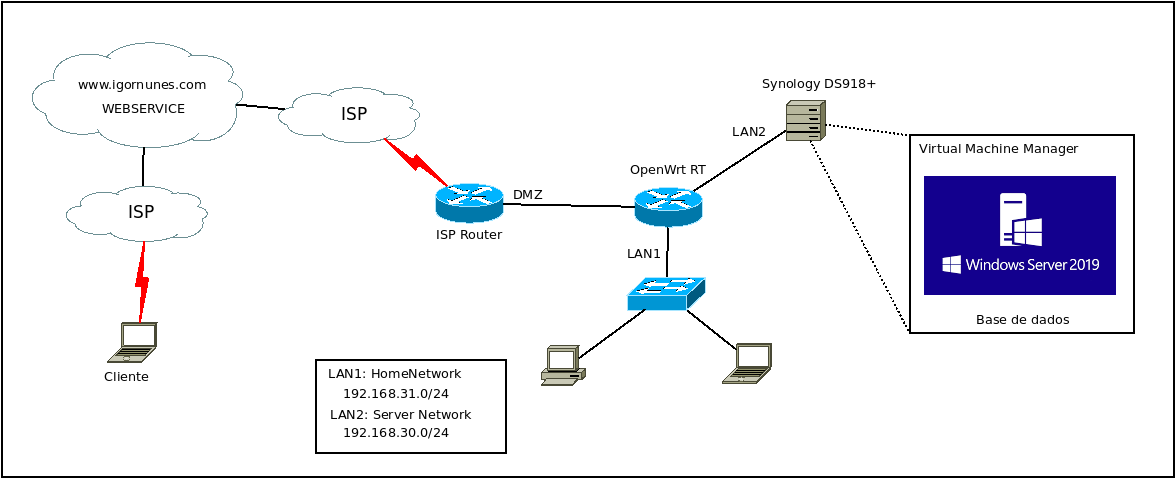
\includegraphics[scale=0.325]{Imagens/DiagramaActual.png}	\caption[Diagrama da arquitetura do sistema atulizado]{Diagrama da arquitetura do sistema atulizado}
	\label{fig::diagrama-sistema-new}
\end{figure}

\section{Reflexão Crítica}
\label{chap4:sec:reflexao}

\subsection{Pontos Fortes}
\label{chap4:subsec:pontosfortes}

\subsection{Pontos Fracos}
\label{chap4:subsec:pontosfracos}

\subsection{Ameaças}
\label{chap4:subsec:ameacas}

\subsection{Oportunidades}
\label{chap4:subsec:oportunidades}

\section{Conclusões}
\label{chap4:sec:concs}
Cada capítulo \underline{intermédio} deve referir o que demais importante se conclui desta parte do trabalho, de modo a fornecer a motivação para o capítulo ou passos seguintes.